\chapter{Controllo di flusso e controllo di congestione}

% ══════════════════════════════════════════════════════════════
\section{Il problema comune: i buffer che traboccano}
% ══════════════════════════════════════════════════════════════

C'è un campo dell'header che non abbiamo mai usato, la finestra di ricezione, e un limite che non sta in nessun header.
\begin{itemize}
    \item La finestra di ricezione dice quanto spazio resta nel buffer all'altro capo: un limite fissato dal
          \textbf{ricevente}.
    \item L'altro limite lo fissa la \textbf{rete}, che non annuncia niente e va indovinato da ciò che torna indietro.
    \item Entrambi finiscono nella stessa azione, inviare di meno, per ragioni che non hanno niente a che vedere l'una con
          l'altra. L'affidabilità ci ha detto che cosa fare dopo una perdita; niente ancora dice come non causarla.
\end{itemize}

Oltre all'affidabilità, TCP offre rispetto a UDP il \textbf{controllo di flusso} e il \textbf{controllo di
congestione}. Entrambi nascono dallo stesso fatto: la perdita di pacchetti su Internet raramente è un cavo rotto, e quasi
sempre è un \textbf{buffer pieno}.

\begin{itemize}
    \item Il \textbf{buffer di ricezione} del destinatario trabocca se l'applicazione non legge i dati abbastanza
          in fretta $\Rightarrow$ problema di \textbf{flusso}.
    \item I \textbf{buffer dei dispositivi di rete} (i router) traboccano se i nodi sono congestionati
          $\Rightarrow$ problema di \textbf{congestione}.
\end{itemize}

\begin{figure}[H]
\centering
\begin{tikzpicture}[every node/.style={font=\footnotesize\sffamily}]
  \draw[thick] (0,0) -- (0,1.4) -- (1.4,1.4) -- (1.4,0); \fill[netblue!50] (0.02,0.02) rectangle (1.38,1.1);
  \node at (0.7,-0.3) {mittente};
  \draw[thick, netblue!70, line width=4pt] (1.4,0.4) -- (4.2,0.4);
  \draw[thick] (4.2,0.6) -- (4.2,1.8) -- (5.6,1.8) -- (5.6,0.6) -- cycle; \fill[netblue!50] (4.22,0.62) rectangle (5.58,1.8);
  \foreach \x in {4.4,4.9,5.3} \fill[netblue!60] (\x,1.85) circle (2pt);
  \node[text=netred] at (4.9,2.3) {trabocca!};
  \node at (4.9,0.3) {router (congestione)};
  \draw[thick, netblue!70, line width=4pt] (5.6,0.9) -- (8.2,0.9);
  \draw[thick] (8.2,0.5) -- (8.2,1.9) -- (9.6,1.9) -- (9.6,0.5) -- cycle; \fill[netblue!50] (8.22,0.52) rectangle (9.58,1.7);
  \draw[thick, netblue!70, line width=1.2pt] (9.6,0.7) -- (10.6,0.7);
  \node[align=center] at (8.9,0.1) {buffer di ricezione\\(flusso)};
  \node[align=center] at (11.2,0.7) {applicazione\\lenta};
\end{tikzpicture}
\caption{L'analogia dell'acqua: i buffer sono secchi intermedi che traboccano se entra più acqua di quanta ne esca.}
\end{figure}

Se i pacchetti si perdono, gli host devono affidarsi a ritrasmissioni e timeout, che curano il sintomo e aggiungono
traffico a una rete che ne aveva già troppo. Meglio evitare di arrivarci.

% ══════════════════════════════════════════════════════════════
\section{Il controllo di flusso}
% ══════════════════════════════════════════════════════════════

Quando TCP riceve byte corretti e in sequenza, li mette nel \textbf{buffer di ricezione}. L'applicazione li
legge da lì, ma non necessariamente nell'istante in cui arrivano (può essere occupata). Se l'applicazione è
lenta a leggere, il mittente può facilmente far traboccare il buffer inviando troppi dati troppo in fretta.

\dfn{Controllo di flusso}{
    Il \textbf{controllo di flusso} di TCP è un servizio di \textbf{adeguamento della velocità}
    (\emph{speed-matching}): cerca di adeguare (ridurre) il ritmo di invio del mittente al ritmo con cui
    l'\textbf{applicazione ricevente} legge i dati. Si basa sulla \textbf{finestra di ricezione}
    (\emph{receive window}, rwnd), il campo dell'header TCP con cui il ricevente comunica al mittente quanto
    spazio libero gli resta nel buffer.
}

\begin{itemize}
    \item Un mittente veloce e un lettore lento fanno traboccare il buffer con una rete che ha fatto tutto giusto.
    \item Anche il controllo di congestione frena il mittente, per una ragione del tutto diversa: i due vengono confusi di
          continuo.
    \item UDP non ha niente di tutto questo: il buffer davanti al socket si riempie e i datagrammi vengono scartati senza
          una parola.
\end{itemize}

\begin{figure}[H]
    \centering
    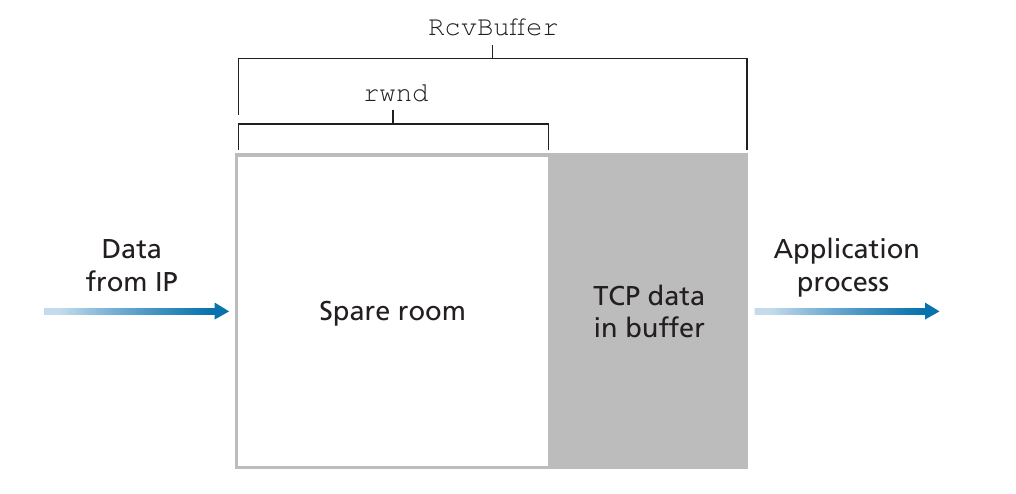
\includegraphics[width=0.55\linewidth]{cap12/rwnd_buffer.png}
    \caption{Il buffer di ricezione: la parte grigia contiene dati non ancora letti dall'applicazione, la parte bianca (rwnd) è lo spazio libero.}
\end{figure}

\subsection{Le formule}

Supponiamo per semplicità che il ricevente scarti i segmenti fuori ordine, così che tutti i dati nel buffer
siano in ordine. Sul \textbf{ricevente} (host B) si definiscono:

\begin{itemize}
    \item \texttt{RcvBuffer}: la dimensione del buffer di ricezione (in byte);
    \item \texttt{LastByteRead}: l'ultimo byte del flusso letto dall'applicazione;
    \item \texttt{LastByteRcvd}: l'ultimo byte del flusso arrivato e messo nel buffer.
\end{itemize}

\dfn{Finestra di ricezione}{
    $$\text{rwnd} = \text{RcvBuffer} - (\text{LastByteRcvd} - \text{LastByteRead})$$
    cioè lo spazio totale meno i byte ricevuti ma non ancora letti.
}

Sul \textbf{mittente} (host A) si tengono \texttt{LastByteSent} (l'ultimo byte inviato) e \texttt{LastByteAcked}
(l'ultimo byte confermato dal ricevente). Conoscendo la finestra comunicata da B, il mittente garantisce in
ogni istante:

$$\text{LastByteSent} - \text{LastByteAcked} \leq \text{rwnd}$$

cioè i byte ``in volo'' (inviati ma non confermati) non superano mai lo spazio libero del ricevente, quindi il buffer
non può traboccare. rwnd cambia ogni volta che uno dei due numeri si muove, quindi va annunciata \textbf{di continuo}: il
ricevente la scrive nel campo finestra di ogni segmento che rimanda indietro. E la connessione è full-duplex: ogni
direzione ha la propria finestra, e ogni estremo ne annuncia una.

\begin{figure}[H]
\centering
\begin{tikzpicture}[every node/.style={font=\scriptsize\sffamily}]
  \foreach \i in {0,...,15} {
    \pgfmathsetmacro{\c}{\i<5 ? "lnet" : (\i<9 ? "llink" : (\i<12 ? "white" : "lphy"))}
    \node[draw, fill=\c, minimum width=0.7cm, minimum height=0.6cm] at (\i*0.7,0) {};
  }
  \draw[decorate, decoration={brace, amplitude=5pt}] (-0.35,0.4) -- (3.15,0.4) node[midway, above=6pt] {inviati e confermati};
  \draw[decorate, decoration={brace, amplitude=5pt}] (3.15,0.4) -- (5.95,0.4) node[midway, above=6pt, align=center] {inviati, non confermati};
  \draw[decorate, decoration={brace, amplitude=5pt}] (5.95,0.4) -- (8.05,0.4) node[midway, above=6pt, align=center] {inviabili};
  \draw[decorate, decoration={brace, amplitude=5pt}] (8.05,0.4) -- (11.2,0.4) node[midway, above=6pt] {non ancora inviabili};
  \draw[decorate, decoration={brace, amplitude=5pt, mirror}] (3.15,-0.4) -- (8.05,-0.4) node[midway, below=6pt, text=netred] {rwnd};
  \node[below=16pt] at (3.15,-0.2) {LastByteAcked};
  \node[below=16pt] at (5.95,-0.9) {LastByteSent};
  \draw[-{Stealth}] (5.95,-1.15) -- (5.95,-0.35);
\end{tikzpicture}
\caption{Lato mittente: il flusso di byte e la finestra consentita dal ricevente.}
\end{figure}

\begin{esempio}{Calcolare la finestra}
B ha un buffer da 4000 byte. Ha ricevuto fino al byte 3000 (\texttt{LastByteRcvd} = 3000) e l'applicazione ha letto
fino al byte 1000 (\texttt{LastByteRead} = 1000). Allora:
$$\text{rwnd} = 4000 - (3000 - 1000) = 2000 \text{ byte}$$
B scrive 2000 nel campo finestra dei segmenti che invia ad A. Se A ha già inviato fino al byte 3500 e ha ricevuto
conferma fino al 3000, ha 500 byte in volo e può inviarne ancora al massimo $2000 - 500 = 1500$.
\end{esempio}

\warning{Finestra a zero}{
    Se il buffer di B si riempie, B comunica $\text{rwnd} = 0$ e A si ferma. Ma se B non ha dati da inviare, non
    manderà più segmenti, e A non saprebbe mai che si è liberato spazio! Per evitare il blocco, quando la finestra è
    zero il mittente continua a inviare periodicamente segmenti di \textbf{un byte} (\emph{zero window probe}): le
    risposte di B contengono il valore aggiornato della finestra. Sono le \textbf{sonde di finestra}, e si vedono in una
    cattura: un trasferimento fermo non è un trasferimento silenzioso.
}

\subsection{Sedici bit non bastano più}

\begin{itemize}
    \item Il campo contiene al massimo 65\,535: la finestra più grande che un ricevente possa annunciare è 64 KB.
    \item Una finestra è anche un \textbf{limite di velocità}: al massimo una finestra per andata e ritorno, quindi al
          massimo $\text{finestra}/\text{RTT}$. 64 KB su un percorso da 100 ms sono circa 5 Mb/s, qualunque cosa valga il
          collegamento sotto.
    \item Il \textbf{prodotto banda-ritardo} dice quanto deve stare in volo per riempire il tubo: 1 Gb/s sullo stesso
          percorso sono 12,5 MB in volo, duecento volte il campo.
    \item Per questo l'opzione \key{window scale} porta un numero di bit di cui spostare il valore, concordato nei due
          segmenti SYN e mai più. Il numero nel campo non è la finestra: va spostato, e una cattura che ha perso l'handshake
          non può sapere di quanto.
\end{itemize}

% ══════════════════════════════════════════════════════════════
\section{Il problema della congestione}
% ══════════════════════════════════════════════════════════════

Il problema della congestione è simile a quello del flusso, ma riguarda l'\textbf{infrastruttura di rete}
invece del ricevente.
\begin{itemize}
    \item Il controllo di flusso è un accordo fra i due estremi: la rete non ne fa parte e non vi compare.
    \item Ma il percorso è condiviso: un mittente può stare ben dentro la finestra del ricevente e immettere comunque più di
          quanto il percorso porti.
    \item E \textbf{nessuno lo dice}: i router non mandano lamentele, e nessuno dei due estremi vede la coda che si sta
          riempiendo.
\end{itemize}
Due domande: che cosa costa davvero la congestione, e come fa un mittente ad accorgersene? Alla prima rispondono tre
scenari, e la risposta peggiora ogni volta.

\subsection{Scenario 1: buffer infinito}

\begin{figure}[H]
    \centering
    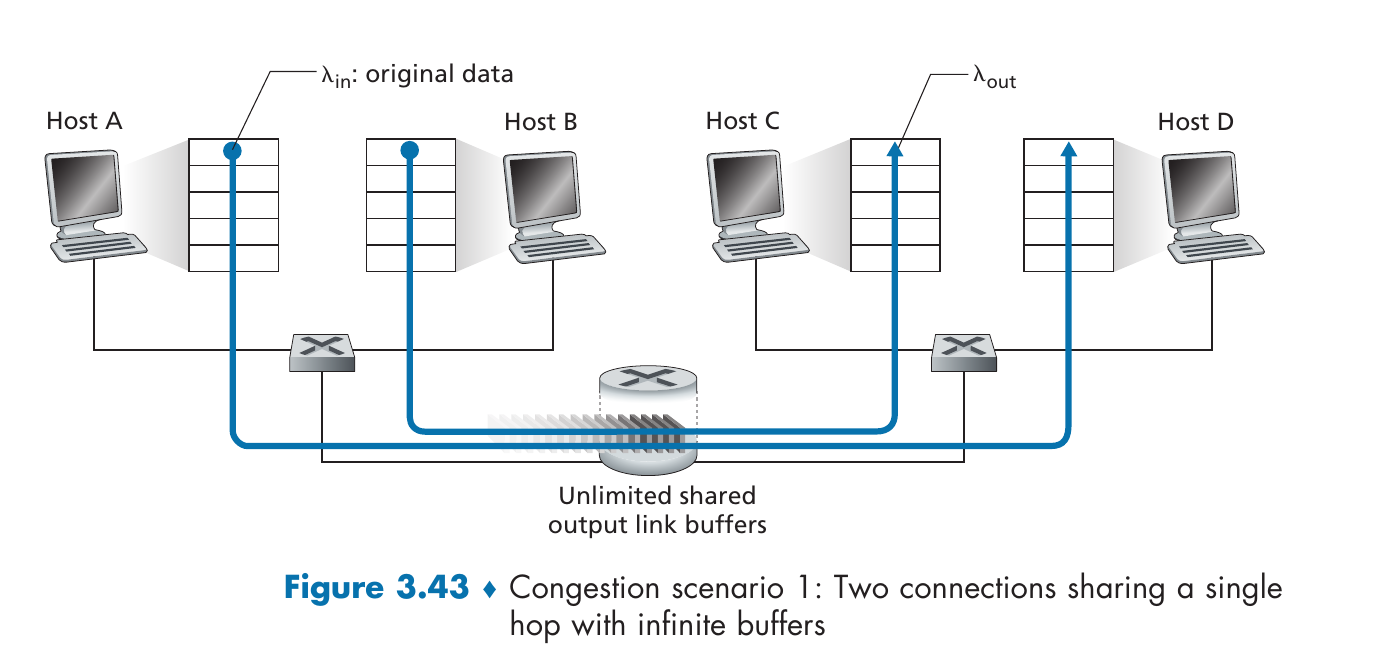
\includegraphics[width=0.55\linewidth]{cap12/scenario1.png}
    \caption{Due connessioni condividono un solo router con buffer infinito e un collegamento in uscita di capacità $R$.}
\end{figure}

Due host (A e B) hanno ciascuno una connessione che attraversa lo stesso router e lo stesso collegamento
in uscita di capacità $R$. Il router ha dei buffer che conservano i pacchetti quando la velocità di arrivo
supera la capacità del collegamento. Entrambe le applicazioni inviano dati alla stessa velocità media di
$\lambda_{in}$ byte/s.

\begin{figure}[H]
    \centering
    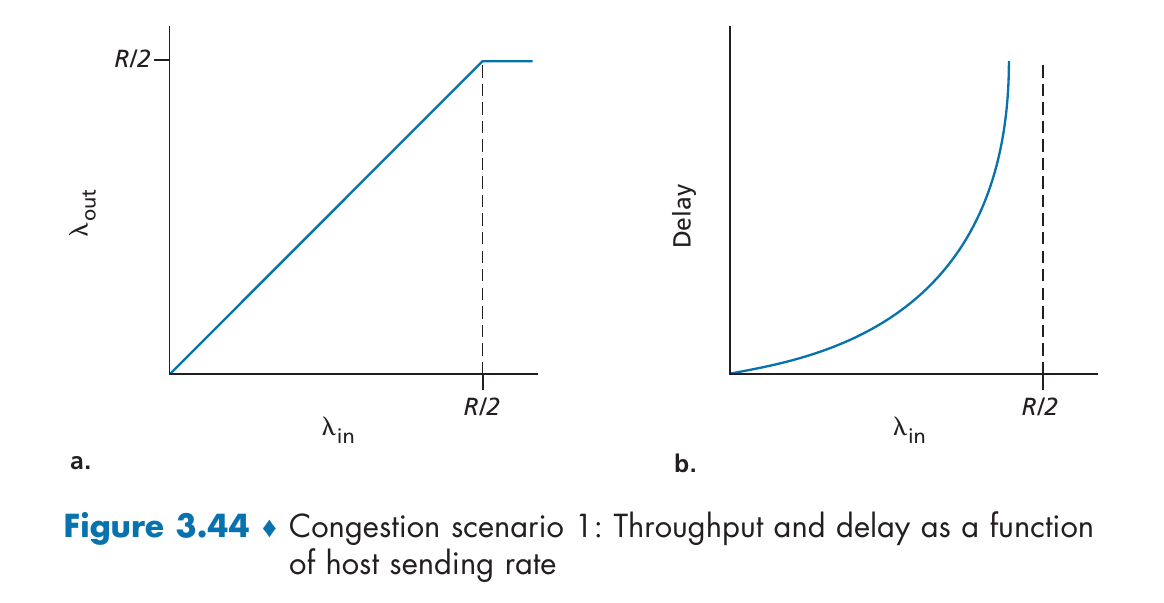
\includegraphics[width=0.6\linewidth]{cap12/scenario1_grafici.png}
    \caption{(a) Throughput per connessione in funzione della velocità di invio: non supera $R/2$. (b) Ritardo: cresce senza limite avvicinandosi a $R/2$.}
\end{figure}

Qui il trasporto non fa niente: nessuna ritrasmissione, nessun controllo di flusso o di congestione. I router sono
store-and-forward, quindi hanno buffer, e in questo primo scenario i buffer sono infiniti: non si scarta mai niente.

\begin{itemize}
    \item Se $\lambda_{in} < R/2$, tutto ciò che il mittente invia arriva al ricevente con un ritardo finito.
    \item Se $\lambda_{in} = R/2$, il collegamento lavora a piena capacità ($R$), e i pacchetti in eccesso finiscono nel buffer.
    \item Finché si supera la capacità, i pacchetti si accumulano nel buffer in attesa del loro turno.
    \item Anche un buffer \textbf{infinito} non basta: i pacchetti non vengono persi, ma il \textbf{ritardo} cresce
          continuamente; se si supera la capacità per sempre, il ritardo tende all'infinito, e i pacchetti sono come persi.
\end{itemize}
Qui non si perde niente: le code da sole, senza alcuna perdita, rendono già inutilizzabile un collegamento vicino alla
capacità.

\subsection{Scenario 2: buffer finito e ritrasmissioni}

\begin{figure}[H]
    \centering
    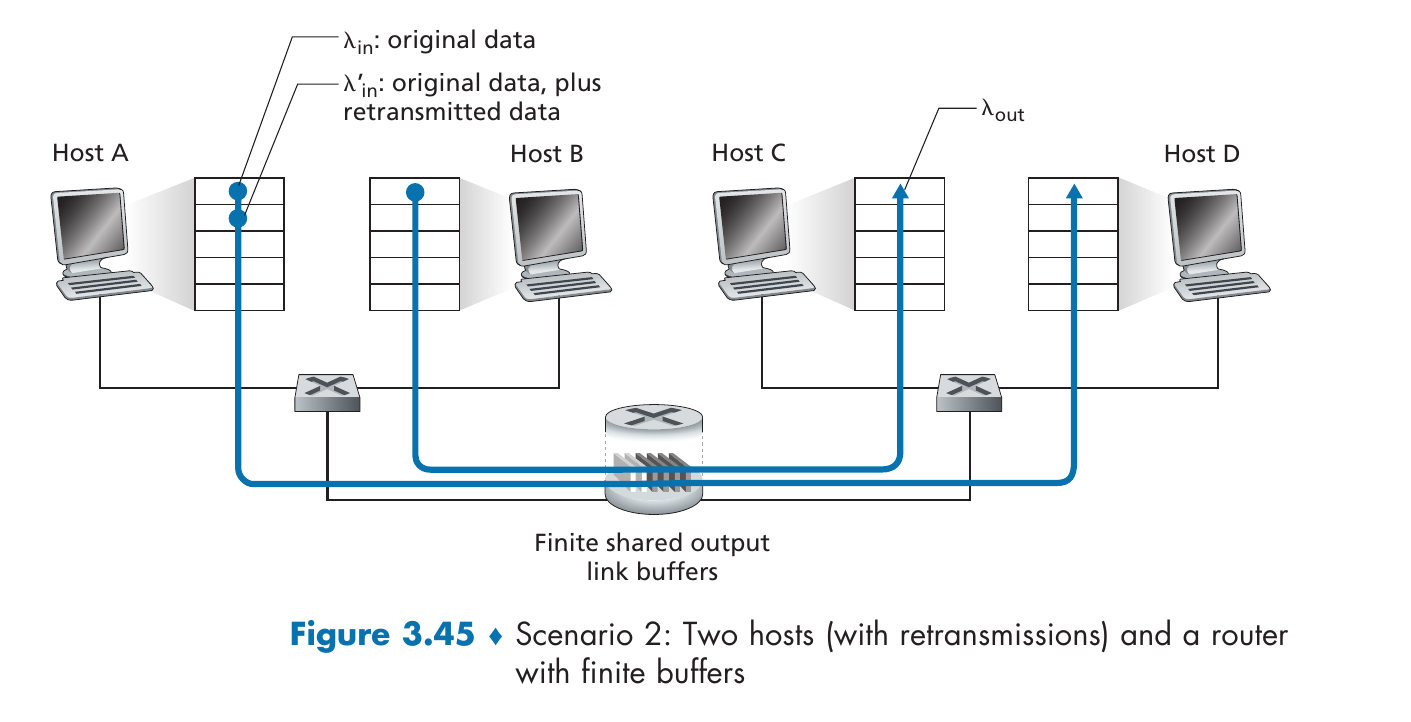
\includegraphics[width=0.55\linewidth]{cap12/scenario2.png}
    \caption{Lo stesso scenario con un buffer finito: i pacchetti in eccesso vengono scartati e i mittenti ritrasmettono.}
\end{figure}

Poiché il buffer è finito, i pacchetti accumulati prima o poi vengono \textbf{scartati}, e gli host devono
\textbf{ritrasmetterli}: altro traffico che si aggiunge a quello già eccessivo. Ora le velocità sono tre invece di una:
\begin{itemize}
    \item $\lambda_{in}$: i dati \textbf{originali}, ciò che l'applicazione consegna al socket;
    \item $\lambda'_{in}$: il \textbf{carico offerto}, dati originali più ritrasmissioni, cioè ciò che vede davvero il
          collegamento;
    \item $\lambda_{out}$: ciò che viene consegnato all'altro capo.
\end{itemize}
Nel primo scenario erano lo stesso numero. Ora non lo sono più, e le differenze fra loro sono il costo.

\begin{figure}[H]
    \centering
    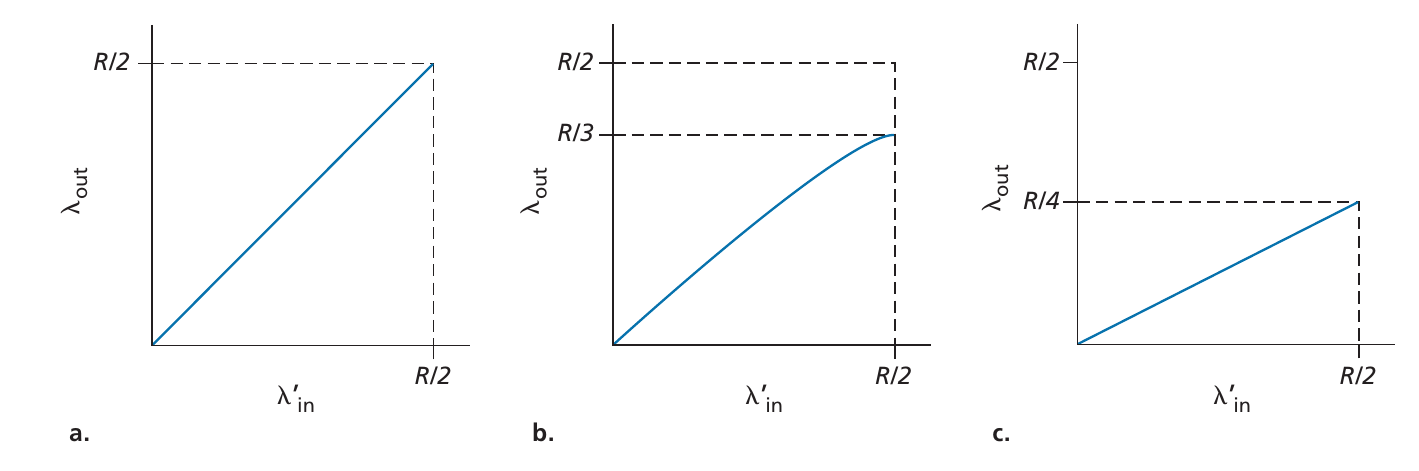
\includegraphics[width=0.6\linewidth]{cap12/scenario2_grafici.png}
    \caption{(a) Ritrasmissioni solo dei pacchetti davvero persi: si arriva a $R/2$. (b) Parte della capacità va in ritrasmissioni: il throughput utile scende (per esempio a $R/3$). (c) Con timeout prematuri si ritrasmettono anche pacchetti non persi: il throughput utile scende ancora (per esempio a $R/4$).}
\end{figure}

\begin{itemize}
    \item (a) Un mittente che sapesse magicamente quando c'è posto nel buffer: non si perde niente, e ciò che si offre viene
          consegnato.
    \item (b) Ritrasmettendo solo ciò che si è davvero perso: con un carico offerto di $R/2$ solo $R/3$ sono dati utili, il
          resto del collegamento trasporta seconde copie.
    \item (c) Con timer che scattano troppo presto ogni pacchetto viene inoltrato in media due volte, e la parte utile scende
          a $R/4$. ($R/3$ e $R/4$ sono valori d'esempio: ciò che mostrano è il degrado, non una costante.)
\end{itemize}

\subsection{Scenario 3: la perdita al secondo salto}

\begin{itemize}
    \item Ora i mittenti sono quattro, su percorsi di due salti che si sovrappongono: ogni connessione compete con una diversa
          a ciascun router.
    \item Il traffico che ha già attraversato il primo router deve lottare per un posto nel buffer del secondo.
    \item Al crescere del carico offerto il throughput di una connessione non si livella: \textbf{scende}, e al limite va a
          zero.
    \item Il costo peggiore: quando un pacchetto viene scartato al secondo salto, tutta la capacità spesa per portarlo fin lì
          è sprecata. Il primo router avrebbe fatto meglio a restare fermo.
\end{itemize}

\begin{figure}[H]
\centering
\begin{tikzpicture}[every node/.style={font=\scriptsize\sffamily}]
  \draw[-{Stealth[length=2mm]}, thick] (0,0) -- (5.2,0) node[right]{$\lambda'_{in}$};
  \draw[-{Stealth[length=2mm]}, thick] (0,0) -- (0,2.8) node[above]{$\lambda_{out}$};
  \draw[dashed, black!40] (0,2.2) node[left, text=black]{$R/2$} -- (5,2.2);
  \draw[very thick, netblue] plot[smooth] coordinates {(0,0) (0.8,0.75) (1.5,1.25) (2.1,1.4) (2.8,1.15) (3.6,0.6) (4.4,0.25) (5,0.1)};
  \node[align=center, text=netred, anchor=west] at (3.0,1.6) {collasso:\\più si offre,\\meno arriva};
\end{tikzpicture}
\caption{Il throughput di una connessione nello scenario a più salti: oltre un certo carico offerto cala fino a zero.}
\end{figure}

\dfn{Collasso da congestione}{
    Il \textbf{collasso da congestione} è lo stato in cui la rete è piena di pacchetti che verranno scartati prima di
    arrivare: lavora al massimo e consegna quasi niente. È successo a Internet reale, alla fine degli anni Ottanta, e
    tutto ciò che segue in questo capitolo è stato scritto in risposta.
}

\warning{I costi della congestione}{
    \begin{itemize}
      \item \textbf{Ritardi} di accodamento elevati quando la velocità di arrivo si avvicina alla capacità.
      \item Il mittente deve \textbf{ritrasmettere} i pacchetti scartati, sprecando capacità.
      \item Timeout prematuri causano ritrasmissioni di pacchetti \textbf{non persi}: altro spreco.
      \item Un pacchetto scartato a metà cammino ha sprecato la capacità di tutti i collegamenti già attraversati.
    \end{itemize}
}

% ══════════════════════════════════════════════════════════════
\section{I due approcci al controllo di congestione}
% ══════════════════════════════════════════════════════════════

\begin{enumerate}
    \item \textbf{Controllo end-to-end}: è l'approccio standard di TCP. La congestione è \textbf{dedotta} dai sistemi
          terminali osservando il comportamento della rete (perdite, ritardi), senza alcun aiuto dal livello di rete: è
          ciò che impone IP, che non offre alcun riscontro. La perdita di un segmento (timeout o 3 ACK duplicati) è presa
          come segnale di congestione, e TCP riduce la velocità di invio.
    \item \textbf{Controllo assistito dalla rete}: approccio più recente e facoltativo, in cui trasporto e rete
          collaborano. I \textbf{router} forniscono un riscontro esplicito sullo stato di congestione: il mittente viene
          informato invece di dover indovinare. Il messaggio può tornare direttamente al mittente (un \emph{choke packet}),
          oppure proseguire come un segno su un pacchetto, che il ricevente poi rimanda indietro. Il secondo modo costa
          un'intera andata e ritorno, ed è quello che Internet ha adottato.
\end{enumerate}

\subsection{ECN: due bit e due flag}

\begin{itemize}
    \item Due bit nell'header IP la portano: un valore dice che entrambi gli estremi sanno gestire ECN, un altro dice
          «questo router è congestionato».
    \item Il router congestionato \textbf{non scarta niente}: marca un datagramma che è già in viaggio verso il ricevente.
    \item Il TCP ricevente gira il segno e accende \textbf{ECE} in una conferma diretta al mittente.
    \item Il mittente dimezza la finestra come se si fosse perso un segmento, e accende \textbf{CWR} nel segmento successivo
          per dire che l'ha fatto.
    \item Il punto: il segnale può arrivare \textbf{prima} della perdita, quindi il costo degli scenari precedenti non si
          paga mai. Funziona solo se i due estremi e i router in mezzo sono tutti d'accordo a usarlo.
\end{itemize}

% ══════════════════════════════════════════════════════════════
\section{Il controllo di congestione di TCP}
% ══════════════════════════════════════════════════════════════

TCP usa soprattutto il controllo \textbf{end-to-end}: ogni mittente adatta la propria velocità alla
congestione che percepisce. I problemi da risolvere sono tre:

\begin{enumerate}
    \item \textbf{Regolazione del ritmo}: come fa il mittente a limitare la velocità a cui immette traffico nella connessione?
    \item \textbf{Rilevazione della congestione}: come fa ad accorgersi che c'è congestione tra sé e la destinazione?
    \item \textbf{Aggiustamento del ritmo}: con quale algoritmo cambia la velocità in funzione della congestione percepita?
\end{enumerate}
E il vincolo dietro a tutte e tre: i mittenti \textbf{non sono coordinati}. Ognuno agisce su informazioni locali, in modo
asincrono.

\subsection{1. Regolazione del ritmo: la congestion window}

Nel controllo di flusso il ritmo è regolato dallo spazio del ricevente
($\text{LastByteSent} - \text{LastByteAcked} \leq \text{rwnd}$). Nel controllo di congestione il mittente
tiene anche una \textbf{finestra di congestione} (\emph{congestion window}, cwnd).

\dfn{Congestion window}{
    $$\text{LastByteSent} - \text{LastByteAcked} \leq \min\{\text{cwnd},\ \text{rwnd}\}$$
    Il ritmo di invio viene regolato \textbf{aumentando o diminuendo cwnd}: più grande è la finestra, più byte si
    possono avere in volo, più veloce è la trasmissione.
}

\begin{figure}[H]
\centering
\begin{tikzpicture}[every node/.style={font=\scriptsize\sffamily}]
  \fill[lnet] (0,0) rectangle (3,0.6); \fill[llink] (3,0) rectangle (6,0.6); \fill[white] (6,0) rectangle (8,0.6); \fill[lphy] (8,0) rectangle (12,0.6);
  \foreach \x in {0,0.5,...,12} \draw (\x,0) -- (\x,0.6);
  \draw (0,0) rectangle (12,0.6);
  \node[above] at (1.5,0.6) {inviati e confermati}; \node[above] at (4.5,0.6) {inviati, non confermati};
  \node[above] at (7,0.6) {inviabili}; \node[above] at (10,0.6) {non inviabili};
  \draw[{Stealth}-{Stealth}, very thick, netred] (3,-0.3) -- node[below, text=netred] {cwnd} (8,-0.3);
  \draw[{Stealth}-{Stealth}, very thick, netblue] (3,-0.9) -- node[below, text=netblue] {rwnd} (10,-0.9);
  \node[anchor=west, text width=4cm] at (12.3,-0.6) {la finestra effettiva è la più piccola delle due};
\end{tikzpicture}
\caption{Congestion window e receive window: comanda la più restrittiva.}
\end{figure}

cwnd non sta in nessun header: il ricevente non la conosce mai. Approssimativamente, all'inizio di ogni andata e ritorno il
mittente può immettere cwnd byte, e alla fine sono stati confermati; la velocità di invio è quindi circa
\[ \text{velocità} \approx \frac{\text{cwnd}}{\text{RTT}} \ \text{byte/s} \]
e cambiare la finestra è l'unico modo che il mittente ha per cambiarla.

\subsection{2. Rilevazione della congestione: i loss event}

\dfn{Loss event}{
    Il mittente TCP percepisce la congestione attraverso gli \textbf{eventi di perdita} (\emph{loss event}):
    \begin{itemize}
      \item la scadenza di un \textbf{timeout};
      \item la ricezione di \textbf{3 ACK duplicati}.
    \end{itemize}
    Entrambi indicano che un pacchetto precedente non è arrivato, probabilmente per il traboccare di un buffer in rete.
}

\begin{itemize}
    \item Un evento di perdita sono in tutto quattro conferme per lo stesso byte (l'originale e tre duplicati), oppure un
          timeout. Entrambi significano un datagramma scartato, e un datagramma scartato significa quasi sempre un buffer
          pieno in un router: il mittente lo legge come un'affermazione sul \textbf{percorso}, non sul cavo o sul ricevente.
    \item Se \textbf{non} ci sono eventi di perdita, cioè gli ACK arrivano come previsto, TCP assume che la rete non
          sia congestionata e \textbf{aumenta} cwnd. Gli ACK che arrivano fanno da ``orologio'': più arrivano in
          fretta, più in fretta cresce la finestra (TCP è \emph{self-clocking}). Un percorso che restituisce le conferme
          lentamente apre quindi lentamente la finestra, senza che nessuno lo decida; e due connessioni con andate e
          ritorni diversi attraverso lo stesso collo di bottiglia non crescono alla stessa velocità.
    \item Se ci sono eventi di perdita, cwnd va \textbf{diminuita}.
    \item Si noti che cosa \textbf{non} si usa: nessuna misura del ritardo, e nessun messaggio da alcun router. Solo i due
          eventi.
\end{itemize}

\subsection{3. Aggiustamento del ritmo: l'algoritmo di Jacobson}

L'aggiustamento avviene tramite il \textbf{sondaggio della banda} (\emph{bandwidth probing}): non c'è una velocità
giusta da calcolare. Il mittente aumenta finché fa male, arretra, e ricomincia ad aumentare: il ritmo cresce finché gli ACK
arrivano correttamente (si ``tasta'' la rete), e quando si rileva congestione (eventi di perdita) viene ridotto. Il
processo si ripete all'infinito.

TCP usa l'algoritmo di controllo di congestione di \textbf{Jacobson} (1988), con tre fasi:

\begin{enumerate}
    \item \textbf{Slow start}: si parte da 1 MSS e la velocità cresce \textbf{esponenzialmente}.
    \item \textbf{Additive increase} (o \emph{congestion avoidance}): la velocità cresce \textbf{linearmente}.
    \item \textbf{Fast recovery} (raccomandata): dopo 3 ACK duplicati si \textbf{dimezza} la velocità invece di
          ripartire da capo, e si prosegue con l'incremento lineare.
\end{enumerate}
Le prime due sono obbligatorie; la terza è raccomandata, ed è ciò che separa le due versioni di TCP che tutti citano.

% ══════════════════════════════════════════════════════════════
\section{Le fasi dell'algoritmo}
% ══════════════════════════════════════════════════════════════

\subsection{Slow start}

\dfn{Slow start}{
    All'inizio della connessione $\text{cwnd} = 1$ MSS. Per ogni ACK ricevuto cwnd aumenta di 1 MSS: così la finestra
    \textbf{raddoppia a ogni RTT} (1, 2, 4, 8, \dots). Nonostante il nome, la crescita è esponenziale: ``lento'' è solo il
    punto di partenza.
}

\begin{figure}[H]
\centering
\begin{tikzpicture}[yscale=0.62, every node/.style={font=\scriptsize\sffamily}]
  \timeline{a}{0}{Host A}{8.2}
  \timeline{b}{4}{Host B}{8.2}
  \draw[msg, netblue] (0,-0.2) -- node[above, sloped] {1 segmento} (4,-0.9);
  \draw[msg, netgreen] (4,-1.0) -- (0,-1.7);
  \draw[msg, netblue] (0,-1.9) -- (4,-2.6); \draw[msg, netblue] (0,-2.2) -- node[below, sloped] {2 segmenti} (4,-2.9);
  \draw[msg, netgreen] (4,-3.0) -- (0,-3.7); \draw[msg, netgreen] (4,-3.3) -- (0,-4.0);
  \foreach \k in {0,1,2,3} \draw[msg, netblue] (0,-4.2-\k*0.3) -- (4,-4.9-\k*0.3);
  \node[text=netblue] at (2.5,-6.3) {4 segmenti};
  \node[anchor=east] at (-0.3,-0.2) {cwnd = 1}; \node[anchor=east] at (-0.3,-1.9) {cwnd = 2}; \node[anchor=east] at (-0.3,-4.2) {cwnd = 4};
  \draw[decorate, decoration={brace, amplitude=4pt}] (4.3,-0.2) -- (4.3,-1.9) node[midway, right=5pt] {1 RTT};
\end{tikzpicture}
\caption{Slow start: ogni ACK fa crescere cwnd di 1 MSS, quindi la finestra raddoppia a ogni RTT.}
\end{figure}

Con una MSS di 500 byte e un percorso da 200 ms, 1 MSS sono circa 20 kb/s: troppo poco, e il mittente non ha idea di
quanto. La crescita è lineare nelle conferme ed esponenziale nel tempo: ciò che è lento è il punto di partenza, non la
crescita. La crescita esponenziale termina in esattamente tre modi:

\begin{itemize}
    \item si verifica un \textbf{timeout}: si pone $\text{ssthresh} = \text{cwnd}/2$ (la \emph{slow start threshold},
          soglia di slow start), $\text{cwnd} = 1$ MSS, e si ricomincia lo slow start;
    \item cwnd raggiunge \textbf{ssthresh}: si passa in \textbf{congestion avoidance}, perché continuare a raddoppiare
          sarebbe imprudente;
    \item arrivano \textbf{3 ACK duplicati}: si esegue la ritrasmissione veloce e si entra in \textbf{fast recovery}.
\end{itemize}

\textbf{ssthresh} è la memoria di dove ha fatto male l'ultima volta. Parte grande, 64 KB, perché all'inizio non c'è
alcuna memoria; ogni evento di perdita la riscrive, sempre come metà della finestra in uso quando la perdita è stata
rilevata.

\subsection{Congestion avoidance}

\dfn{Congestion avoidance (additive increase)}{
    Invece di raddoppiare, cwnd cresce di \textbf{1 MSS per ogni RTT} (in pratica, di
    $\text{MSS}\cdot\frac{\text{MSS}}{\text{cwnd}}$ per ogni ACK ricevuto). La crescita è \textbf{lineare}.
}

All'ingresso cwnd è circa la metà di quanto era al momento della perdita: il guaio è vicino, e la prudenza è voluta.
Verifica: con $\text{cwnd} = 10$ MSS arrivano dieci conferme in un'andata e ritorno, e ognuna aggiunge un decimo: un MSS in
tutto. Più grande è la finestra, più piccolo è ogni passo, ed è questo che mantiene la crescita lineare nel tempo invece che
esponenziale.

\begin{itemize}
    \item Se scade un \textbf{timeout}: come nello slow start, $\text{ssthresh} = \text{cwnd}/2$, $\text{cwnd} = 1$ MSS, e si torna in slow start.
    \item Se arrivano \textbf{3 ACK duplicati}: la rete riesce ancora a consegnare qualche segmento (gli ACK arrivano),
          quindi la reazione è meno drastica: $\text{ssthresh} = \text{cwnd}/2$, $\text{cwnd} = \text{ssthresh} + 3$ MSS
          (i tre segmenti che hanno generato i duplicati sono usciti dalla rete), e si entra in \textbf{fast recovery}.
\end{itemize}

\warning{Due perdite, due reazioni}{
    Entrambi sono eventi di perdita. Perché un timeout riporta cwnd a 1 MSS, mentre tre conferme duplicate la dimezzano
    soltanto? Perché tre duplicati sono la \textbf{prova che la rete sta ancora consegnando}: i segmenti dopo quello
    mancante sono passati, e qualcosa è tornato a dirlo. Un timeout è silenzio, e il silenzio può significare qualsiasi
    cosa. Per questo la reazione al timeout è quella drastica, e quella ai tre duplicati tiene metà della finestra e
    prosegue da lì.
}

\subsection{Fast recovery}

\dfn{Fast recovery}{
    In \textbf{fast recovery} cwnd aumenta di 1 MSS per ogni ulteriore ACK duplicato ricevuto per il segmento
    mancante. Quando arriva l'ACK del segmento perso, si pone $\text{cwnd} = \text{ssthresh}$ e si torna in
    \textbf{congestion avoidance}. Se invece scade un timeout, si abbandona tutto: si torna in slow start con
    $\text{cwnd} = 1$ MSS.
}

Il $+3$ non è decorativo: tre duplicati significano che tre segmenti hanno lasciato la rete e sono arrivati. Ogni
duplicato successivo aggiunge un altro MSS per la stessa ragione: il tubo si sta svuotando mentre il mittente aspetta.

\info{Tahoe e Reno}{
    La prima versione di TCP con controllo di congestione, \textbf{TCP Tahoe}, non aveva la fast recovery: dopo
    \emph{qualsiasi} evento di perdita ripartiva da $\text{cwnd} = 1$ MSS. \textbf{TCP Reno} ha introdotto la fast
    recovery, che dopo 3 ACK duplicati dimezza la finestra invece di azzerarla.
}

\begin{figure}[H]
\centering
\begin{tikzpicture}
  \begin{axis}[width=12cm, height=6.2cm, xlabel={tempo (RTT)}, ylabel={cwnd (in MSS)}, xmin=0.5, xmax=15.5, ymin=0, ymax=16,
      xtick={1,...,15}, ytick={0,2,...,16}, grid=major, grid style={gray!20}, legend pos=north west,
      legend style={font=\scriptsize\sffamily}, tick label style={font=\scriptsize}, label style={font=\footnotesize\sffamily}]
    \addplot[very thick, netred, mark=*, mark size=1.5pt] coordinates {(1,1) (2,2) (3,4) (4,8) (5,9) (6,10) (7,11) (8,12) (9,1) (10,2) (11,4) (12,6) (13,7) (14,8) (15,9)};
    \addlegendentry{TCP Tahoe}
    \addplot[very thick, netblue, mark=square*, mark size=1.5pt] coordinates {(1,1) (2,2) (3,4) (4,8) (5,9) (6,10) (7,11) (8,12) (9,9) (10,10) (11,11) (12,12) (13,13) (14,14) (15,15)};
    \addlegendentry{TCP Reno}
    \addplot[dashed, black!60, domain=0.5:8.5] {8};
    \addplot[dashed, black!60, domain=8.5:15.5] {6};
    \node[font=\scriptsize\sffamily, anchor=south west] at (axis cs:0.6,8) {ssthresh = 8};
    \node[font=\scriptsize\sffamily, anchor=north east] at (axis cs:15.4,6) {ssthresh = 6};
    \draw[-{Stealth}, thick] (axis cs:8,14.5) -- (axis cs:8,12.6);
    \node[font=\scriptsize\sffamily, anchor=south] at (axis cs:8,14.5) {3 ACK duplicati};
  \end{axis}
\end{tikzpicture}
\caption{Evoluzione di cwnd. Slow start fino a ssthresh = 8, poi crescita lineare. All'RTT 8 (cwnd = 12) arrivano 3 ACK duplicati: ssthresh diventa 6. Tahoe riparte da 1 MSS; Reno riparte da $6 + 3 = 9$ MSS e prosegue linearmente.}
\end{figure}

% ══════════════════════════════════════════════════════════════
\section{La macchina a stati del controllo di congestione}
% ══════════════════════════════════════════════════════════════

\begin{figure}[H]
\centering
\begin{tikzpicture}[every node/.style={font=\scriptsize\sffamily}, st/.style={circle, draw, thick, fill=cloudbg, minimum size=2.2cm, align=center, font=\footnotesize\bfseries\sffamily}]
  \node[st] (ss) at (0,0) {slow\\start};
  \node[st] (ca) at (9,0) {congestion\\avoidance};
  \node[st] (fr) at (4.5,-5.2) {fast\\recovery};
  \draw[-{Stealth}, very thick] (-2.6,1.4) node[above, align=center] {inizio:\\cwnd = 1 MSS, ssthresh = 64 kB} -- (ss);
  \draw[-{Stealth}, thick] (ss) to[loop above, looseness=5] node[above, align=center] {nuovo ACK: cwnd = cwnd + MSS} (ss);
  \draw[-{Stealth}, thick] (ca) to[loop above, looseness=5] node[above, align=center] {nuovo ACK: cwnd = cwnd + MSS$\cdot$(MSS/cwnd)} (ca);
  \draw[-{Stealth}, thick] (fr) to[loop below, looseness=5] node[below, align=center] {ACK duplicato: cwnd = cwnd + MSS} (fr);
  \draw[-{Stealth}, thick, netgreen!60!black] ([yshift=0.3cm]ss.east) -- node[above, align=center] {cwnd $\geq$ ssthresh} ([yshift=0.3cm]ca.west);
  \draw[-{Stealth}, thick, netred] ([yshift=-0.3cm]ca.west) -- node[below, align=center] {timeout: ssthresh = cwnd/2,\\cwnd = 1 MSS} ([yshift=-0.3cm]ss.east);
  \draw[-{Stealth}, thick, netorange] (ss.south) -- node[left, align=right] {3 ACK duplicati:\\ssthresh = cwnd/2,\\cwnd = ssthresh + 3 MSS,\\ritrasmette il segmento} (fr.north west);
  \draw[-{Stealth}, thick, netorange] ([xshift=-0.3cm]ca.south) -- node[left, align=right, pos=0.35] {3 ACK duplicati:\\ssthresh = cwnd/2,\\cwnd = ssthresh + 3 MSS} (fr.north east);
  \draw[-{Stealth}, thick, netgreen!60!black] (fr.east) to[out=0, in=-90] node[right, align=left] {nuovo ACK:\\cwnd = ssthresh} ([xshift=0.4cm]ca.south);
  \draw[-{Stealth}, thick, netred] (fr.west) to[out=180, in=-90] node[left, align=right] {timeout:\\ssthresh = cwnd/2,\\cwnd = 1 MSS} ([xshift=-0.4cm]ss.south);
\end{tikzpicture}
\caption{Macchina a stati semplificata del controllo di congestione di TCP Reno.}
\end{figure}

\begin{figure}[H]
    \centering
    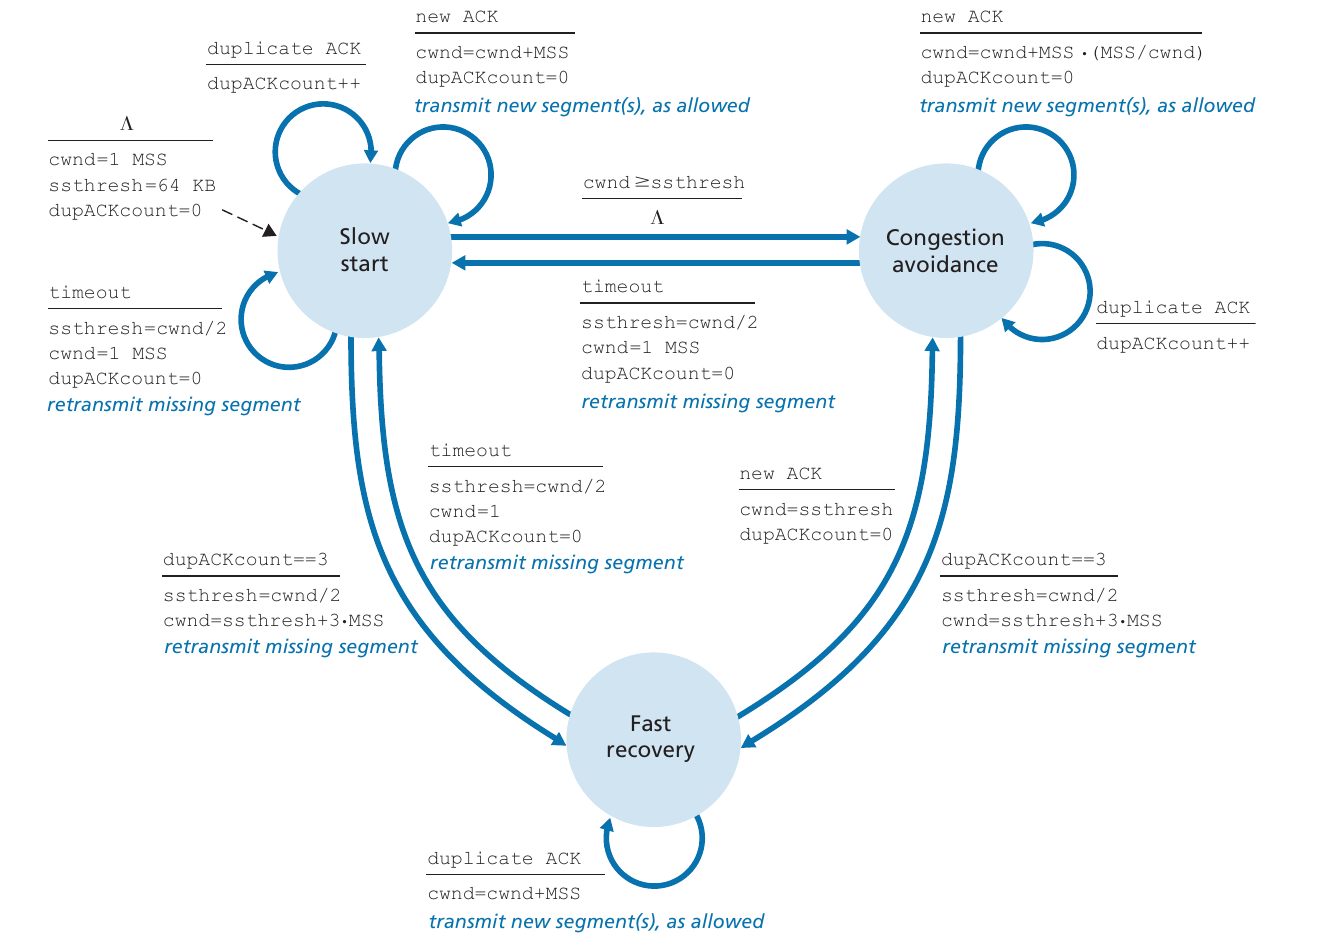
\includegraphics[width=0.62\linewidth]{cap12/fsm_congestione.png}
    \caption{La macchina a stati completa (Kurose), come mostrata a lezione.}
\end{figure}

\subsection{Il quadro completo delle transizioni}

\begin{table}[H]
\centering
\begin{tabular}{p{2.6cm}p{3.4cm}p{4.3cm}p{3.6cm}}
\toprule
\textbf{Stato} & \textbf{Evento} & \textbf{Azione} & \textbf{Nuovo stato} \\
\midrule
Slow start & nuovo ACK & cwnd += MSS & slow start (o CA se cwnd $\geq$ ssthresh) \\
Slow start & 3 ACK duplicati & ssthresh = cwnd/2; cwnd = ssthresh + 3 MSS; ritrasmissione & fast recovery \\
Slow start & timeout & ssthresh = cwnd/2; cwnd = 1 MSS; ritrasmissione & slow start \\
Congestion avoid. & nuovo ACK & cwnd += MSS$\cdot$MSS/cwnd & congestion avoidance \\
Congestion avoid. & 3 ACK duplicati & ssthresh = cwnd/2; cwnd = ssthresh + 3 MSS; ritrasmissione & fast recovery \\
Congestion avoid. & timeout & ssthresh = cwnd/2; cwnd = 1 MSS; ritrasmissione & slow start \\
Fast recovery & ACK duplicato & cwnd += MSS & fast recovery \\
Fast recovery & nuovo ACK & cwnd = ssthresh & congestion avoidance \\
Fast recovery & timeout & ssthresh = cwnd/2; cwnd = 1 MSS & slow start \\
\bottomrule
\end{tabular}
\caption{Tutte le transizioni del controllo di congestione di TCP Reno.}
\end{table}

\info{AIMD e il dente di sega}{
    Ignorando lo slow start iniziale e supponendo le perdite segnalate da 3 ACK duplicati, TCP aumenta cwnd di 1 MSS
    per RTT e la dimezza a ogni perdita: è l'approccio \textbf{AIMD} (\emph{Additive Increase, Multiplicative
    Decrease}). Il grafico di cwnd nel tempo ha la tipica forma a \textbf{dente di sega}. Se $W$ è la finestra a cui
    avviene la perdita, il throughput medio di una connessione è circa $\dfrac{0{,}75\cdot W}{\text{RTT}}$.
}

\begin{figure}[H]
\centering
\begin{tikzpicture}
  \begin{axis}[width=11cm, height=4.6cm, xlabel={tempo}, ylabel={cwnd}, xmin=0, xmax=24, ymin=0, ymax=26, xtick=\empty, ytick={12,24}, yticklabels={$W/2$, $W$},
      tick label style={font=\scriptsize}, label style={font=\footnotesize\sffamily}]
    \addplot[very thick, netblue] coordinates {(0,12) (6,24) (6,12) (12,24) (12,12) (18,24) (18,12) (24,24)};
    \addplot[dashed, netred, domain=0:24] {18};
    \node[font=\scriptsize\sffamily, text=netred, anchor=south east] at (axis cs:24,18) {media $\approx 0{,}75\,W$};
  \end{axis}
\end{tikzpicture}
\caption{Il dente di sega di AIMD: crescita lineare, dimezzamento a ogni perdita.}
\end{figure}

% ══════════════════════════════════════════════════════════════
\section{Che cosa esegue davvero la nostra macchina}
% ══════════════════════════════════════════════════════════════

\begin{itemize}
    \item Reno classico è il \textbf{modello}, non il codice: è ciò che vale la pena capire, e non è ciò che esegue il
          kernel.
    \item \key{CUBIC}: stesso slow start, stessa fast recovery, congestion avoidance diversa: la finestra segue una funzione
          cubica del tempo trascorso dall'ultima perdita. Risale in fretta fino alla finestra che aveva prima della perdita,
          poi sonda con cautela attorno a essa. È il default di Linux.
    \item Basati sul ritardo: \key{Vegas} e \key{BBR} osservano l'andata e ritorno che cresce e rallentano \textbf{prima}
          che si perda qualcosa. L'idea: tenere il tubo appena pieno, ma non di più; un tubo pieno è lavoro utile, una coda
          piena è solo ritardo.
    \item Per la cattura di fine capitolo: il dente di sega che si troverà probabilmente non sarà quello di Reno, e ora si sa
          perché.
\end{itemize}

% ══════════════════════════════════════════════════════════════
\section{Equità}
% ══════════════════════════════════════════════════════════════

\dfn{Equità}{
    Con $K$ connessioni attraverso un collo di bottiglia di rate $R$, il meccanismo è \textbf{equo} se ciascuna finisce
    con circa $R/K$.
}

\begin{figure}[H]
\centering
\begin{tikzpicture}[scale=1.15, every node/.style={font=\scriptsize\sffamily}]
  \draw[-{Stealth[length=2mm]}, thick] (0,0) -- (4.6,0) node[right, align=left]{throughput della\\connessione 1};
  \draw[-{Stealth[length=2mm]}, thick] (0,0) -- (0,4.6) node[above, align=center]{throughput della connessione 2};
  \draw[thick, netgreen!60!black] (4,0) node[below]{$R$} -- (0,4) node[left]{$R$};
  \node[text=netgreen!50!black, rotate=-45] at (2.85,1.4) {piena utilizzazione};
  \draw[dashed, netred] (0,0) -- (3.4,3.4) node[above right, text=netred]{parti uguali};
  \draw[-{Stealth[length=1.5mm]}, netblue, thick] (0.6,1.8) -- (1.4,2.6);
  \draw[-{Stealth[length=1.5mm]}, netblue, thick, dashed] (1.4,2.6) -- (0.7,1.3);
  \draw[-{Stealth[length=1.5mm]}, netblue, thick] (0.7,1.3) -- (1.7,2.3);
  \draw[-{Stealth[length=1.5mm]}, netblue, thick, dashed] (1.7,2.3) -- (0.85,1.15);
  \draw[-{Stealth[length=1.5mm]}, netblue, thick] (0.85,1.15) -- (1.85,2.15);
  \fill[netblue] (0.6,1.8) circle (1.5pt);
  \fill[netred] (2,2) circle (1.8pt);
  \node[anchor=west, align=left, text=netblue] at (4.4,3.0) {aumento additivo:\\a 45 gradi, la differenza resta};
  \node[anchor=west, align=left, text=netblue] at (4.4,2.1) {perdita: entrambi dimezzati,\\verso l'origine};
\end{tikzpicture}
\caption{Due connessioni con la stessa MSS e la stessa andata e ritorno. Ogni ciclo di aumento e dimezzamento avvicina la
         coppia alla bisettrice, e la coppia converge sulla parte uguale da qualunque punto parta.}
\end{figure}

\begin{itemize}
    \item Finché non si perde niente, entrambe aggiungono un MSS per andata e ritorno. Aggiungere la stessa quantità a
          entrambe non cambia la differenza fra loro: la coppia si muove lungo una retta a 45 gradi.
    \item Una perdita dimezza entrambe, e dimezzare due numeri diversi li avvicina: in proporzione, il più grande perde di
          più.
    \item La ragione è che la diminuzione è moltiplicativa e l'aumento no: l'equità è una conseguenza di quell'asimmetria.
\end{itemize}

\warning{E perché l'equità si rompe facilmente}{
    \begin{itemize}
        \item L'argomento assumeva andate e ritorni uguali. Un percorso più corto apre la finestra più in fretta e si prende
              più collegamento, gratis.
        \item UDP non fa niente di tutto questo: non ha finestra, né eventi di perdita, né ragioni per rallentare. Continua a
              inviare. La chat su datagrammi della parte sulla programmazione ritrasmette ciò che si è perso e non riduce mai
              la velocità: è esattamente il flusso iniquo di questa figura.
        \item Nove applicazioni con una connessione ciascuna e una decima con undici: la decima si prende più di metà del
              collegamento ($11/20$), tutto legalmente.
    \end{itemize}
    L'equità di TCP è una \textbf{convenzione fra mittenti}, non una regola che la rete impone.
}

% ══════════════════════════════════════════════════════════════
\section{Che cosa c'è sotto la nostra write}
% ══════════════════════════════════════════════════════════════

\texttt{write} non trasmette: lo avevamo detto quando sono comparsi i due buffer, lasciando aperto il resto. Ecco il
resto.
\begin{itemize}
    \item Copia byte nel buffer di invio e ritorna. TCP li toglie più tardi, secondo il proprio calendario.
    \item Quanti ne possono partire adesso: $\min\{\text{cwnd}, \text{rwnd}\}$, meno ciò che è già in volo. Il buffer si
          svuota quindi alla velocità che il peer e il percorso consentono, e l'applicazione non vede mai nessuno dei due
          numeri.
    \item Una \texttt{write} bloccante ritorna quando c'è posto, quindi \textbf{si blocca quando il buffer è pieno}, cioè
          quando entrambi i limiti sono stati raggiunti.
    \item Una scrittura corta è lo stesso evento a metà: il buffer ha preso parte di ciò che si offriva e si è riempito. Ecco
          perché si cicla. Sui messaggi brevi nessuna delle due cose capita mai, ed è per questo che le si scopre tardi.
\end{itemize}

\warning{Il client che ha smesso di leggere}{
    Un client della chat smette di chiamare \texttt{read}: non è morto, è solo occupato. Che cosa arriva al server? Il suo
    buffer di ricezione si riempie, quindi annuncia $\text{rwnd} = 0$. Il buffer di invio del server si riempie dietro a
    lui, e la \texttt{write} del worker \textbf{si blocca}, tenendo il lock che teneva.
    \begin{itemize}
        \item Niente è rotto e niente è perso: è il controllo di flusso che funziona esattamente come progettato, visto dal
              lato sbagliato.
        \item Sul filo si vede: una finestra che si restringe fino a zero, poi le sonde da un byte, poi un aggiornamento della
              finestra quando il client torna a leggere.
        \item Il bug non è mai stato il client lento: era bloccarsi tenendo il lock della lista, che ha trasformato un client
              silenzioso in una chat congelata.
    \end{itemize}
}

\begin{lstlisting}[language={[POSIX]C}, style=wnumbers, title={EAGAIN, e ciò che non dice}]
ssize_t n = write(fd, out[i].buf, out[i].len);

if (n < 0 && (errno == EAGAIN || errno == EWOULDBLOCK)) {
    FD_SET(fd, &wall);         /* buffer di invio pieno: min(cwnd,rwnd) e' esaurito */
    return;                    /* si torna quando si svuota; nessuno aspetta */
}
if (n < 0 && errno == EINTR) return;    /* un segnale, non uno stallo */
if (n < 0) { drop(i); return; }

out[i].len -= n;               /* anche una scrittura corta arriva qui, ed e' normale */
memmove(out[i].buf, out[i].buf + n, out[i].len);
\end{lstlisting}

\texttt{EAGAIN} dice che il buffer di invio è pieno \textbf{ora}, e niente sul perché. rwnd viaggia in ogni segmento e la
si può leggere in una cattura; cwnd non lascia mai il kernel del mittente. Due cause, un sintomo, e solo una delle due
visibile da fuori.

% ══════════════════════════════════════════════════════════════
\section{Analizzare il traffico TCP con Wireshark}
% ══════════════════════════════════════════════════════════════

La connessione con \texttt{nc} sull'interfaccia di loopback si trova nel capitolo sulla gestione della connessione;
qui si guarda un trasferimento vero, abbastanza lungo da far vedere le finestre al lavoro.

\begin{esercizio}{Uno scaricamento reale da dieci megabyte}
Si avvia \textbf{prima} la cattura, sull'interfaccia davvero in uso, e poi si scarica un file di prova:
\begin{lstlisting}[language=bash]
$ wget http://speedtest.tele2.net/10MB.zip
\end{lstlisting}
Un lungo trasferimento in una sola direzione è la cosa più facile da
leggere: un flusso solo, nessun intreccio, e una dimensione nota. Clic destro su un segmento, \emph{Follow $\rightarrow$
TCP Stream}: Wireshark scrive il filtro \texttt{tcp.stream eq N} e tutto il resto sparisce.
\begin{enumerate}[label=(\alph*)]
    \item Quali quattro numeri sta riassumendo quel filtro, e quale dei quattro non ha scelto nessuno?
    \item \texttt{wget} ha preso la porta del server dall'URL. Si sarebbe potuta scegliere anche la propria porta locale?
    \item In \emph{Statistics $\rightarrow$ TCP Stream Graphs $\rightarrow$ Time/Sequence (tcptrace)}, nella direzione che
          porta i dati: dove finisce la curvatura iniziale? In circa quante andate e ritorno, e che RTT dà al percorso?
    \item Guardare il fattore di window scale nei due SYN: qual è la finestra più grande che ciascun lato potrebbe annunciare?
    \item Trovare una ritrasmissione. È stata preceduta da tre conferme duplicate o da un silenzio? Quale delle due reazioni
          dovrebbe seguire?
    \item Catturare di nuovo con \texttt{wget --limit-rate=200k}. Quale delle due finestre si esaurisce questa volta, e quale
          mai?
\end{enumerate}

\svolgimento
\begin{enumerate}[label=(\alph*)]
    \item Indirizzo e porta del client, indirizzo e porta del server. La porta del client è \textbf{effimera}: l'ha scelta il
          kernel al momento della \texttt{connect}, e nessuno l'ha decisa.
    \item Sì, ma non con \texttt{wget}: un programma può chiamare \texttt{bind} sul socket del client prima di
          \texttt{connect} (con \texttt{nc} c'è l'opzione \texttt{-p}). Di solito non conviene: una porta fissa entra in
          conflitto con le connessioni precedenti ancora in TIME WAIT.
    \item Nel grafico il tempo è in orizzontale e il numero di sequenza in verticale, quindi la pendenza è il throughput. La
          linea bassa sono i dati inviati, quella alta il massimo consentito dal ricevente (conferma più finestra); la distanza
          verticale fra le due è ciò che è in volo. I primi istanti curvano verso l'alto, poi la curva si raddrizza: la
          curvatura è la finestra che si apre (slow start), il tratto dritto è il regime. Contando i «gradini» della curvatura
          (uno per andata e ritorno) e dividendo il tempo che occupano si ottiene una stima dell'RTT, da confrontare con il
          tempo fra SYN e SYNACK.
    \item Il campo è di 16 bit, quindi al massimo $65\,535 \cdot 2^{s}$ byte, dove $s$ è il fattore annunciato nel SYN di
          quel lato (per esempio con $s = 7$, circa 8 MB).
    \item Il filtro \texttt{tcp.analysis.duplicate\_ack} mostra se prima della ritrasmissione ci sono stati tre duplicati:
          allora è una \emph{fast retransmission} e la finestra si dimezza; se invece c'è stato un silenzio è un timeout, e la
          finestra riparte da 1 MSS.
    \item Con il limite di velocità è \texttt{wget} a leggere piano: il buffer di ricezione si riempie e compaiono
          \texttt{tcp.analysis.zero\_window} e \texttt{window\_update}. Si esaurisce \textbf{rwnd}; cwnd non viene mai
          raggiunta, perché il percorso potrebbe portare molto di più di 200 KB/s.
\end{enumerate}
\end{esercizio}

\info{La finestra che si vede, e quella che no}{
    \begin{itemize}
        \item \texttt{tcp.analysis.bytes\_in\_flight}: byte non confermati, pacchetto per pacchetto;
        \item \texttt{tcp.analysis.duplicate\_ack}: il sintomo di una perdita;
        \item \texttt{tcp.analysis.window\_update}: il ricevente che si riapre;
        \item \texttt{tcp.analysis.zero\_window}: il ricevente che non ha più posto.
    \end{itemize}
    Si combinano con \texttt{\&\&} nella barra dei filtri. \texttt{bytes\_in\_flight} è un calcolo di Wireshark su ciò
    che ha visto: coincide con cwnd solo quando il mittente ha sempre dati e rwnd non è la finestra più piccola; altrimenti è
    un limite inferiore. Nella cattura: lo slow start è la curva che piega verso l'alto, con pochi segmenti per andata e
    ritorno; la congestion avoidance una retta, con un ritmo costante di segmenti; la fast recovery conferme duplicate, una
    ritrasmissione, un gradino.
}

\Needspace{20\baselineskip}
% ══════════════════════════════════════════════════════════════
\section{Riepilogo}
% ══════════════════════════════════════════════════════════════

\riepilogo{
\begin{itemize}
    \item \textbf{Flusso}: proteggere il ricevente. $\text{rwnd} = \text{RcvBuffer} - (\text{LastByteRcvd} - \text{LastByteRead})$;
          il mittente mantiene $\text{LastByteSent} - \text{LastByteAcked} \leq \text{rwnd}$.
    \item \textbf{Congestione}: proteggere la rete. Buffer infiniti $\Rightarrow$ ritardi infiniti; buffer finiti $\Rightarrow$
          perdite e ritrasmissioni che sprecano capacità.
    \item TCP usa il controllo \textbf{end-to-end}: $\text{LastByteSent} - \text{LastByteAcked} \leq \min\{\text{cwnd}, \text{rwnd}\}$.
    \item \textbf{Loss event}: timeout o 3 ACK duplicati.
    \item \textbf{Slow start} (cwnd raddoppia per RTT fino a ssthresh), \textbf{congestion avoidance} (+1 MSS per RTT),
          \textbf{fast recovery} (dopo 3 duplicati: ssthresh = cwnd/2, cwnd = ssthresh + 3); timeout $\Rightarrow$ cwnd = 1 MSS.
    \item La congestione costa ritardo prima che perdite, e un pacchetto scartato tardi spreca ogni collegamento che lo ha già
          portato. ECN segnala la congestione prima della perdita.
    \item AIMD rende TCP equo fra connessioni con lo stesso RTT; UDP e le connessioni parallele rompono l'equità, che è una
          convenzione.
    \item La nostra \texttt{write} si blocca, o restituisce \texttt{EAGAIN}, quando $\min\{\text{cwnd}, \text{rwnd}\}$ non ha
          più niente da dare. Prossimo argomento: i router, delle cui code abbiamo parlato fin qui.
\end{itemize}
}
